%% bare_jrnl.tex
%% V1.3
%% 2007/01/11
%% by Michael Shell
%% see http://www.michaelshell.org/
%% for current contact information.
%%
%% This is a skeleton file demonstrating the use of IEEEtran.cls
%% (requires IEEEtran.cls version 1.7 or later) with an IEEE journal paper.
%%
%% Support sites:
%% http://www.michaelshell.org/tex/ieeetran/
%% http://www.ctan.org/tex-archive/macros/latex/contrib/IEEEtran/
%% and
%% http://www.ieee.org/




\documentclass[journal]{IEEEtran}
\usepackage{blindtext}
\usepackage{graphicx}


% *** CITATION PACKAGES ***
%
\usepackage{cite}

% *** GRAPHICS RELATED PACKAGES ***
%
\ifCLASSINFOpdf
  % \usepackage[pdftex]{graphicx}
  % declare the path(s) where your graphic files are
  % \graphicspath{{../pdf/}{../jpeg/}}
  % and their extensions so you won't have to specify these with
  % every instance of \includegraphics
  % \DeclareGraphicsExtensions{.pdf,.jpeg,.png}
\else
  % or other class option (dvipsone, dvipdf, if not using dvips). graphicx
  % will default to the driver specified in the system graphics.cfg if no
  % driver is specified.
  % \usepackage[dvips]{graphicx}
  % declare the path(s) where your graphic files are
  % \graphicspath{{../eps/}}
  % and their extensions so you won't have to specify these with
  % every instance of \includegraphics
  % \DeclareGraphicsExtensions{.eps}
\fi
% graphicx was written by David Carlisle and Sebastian Rahtz. It is
% required if you want graphics, photos, etc. graphicx.sty is already
% installed on most LaTeX systems. The latest version and documentation can
% be obtained at: 
% http://www.ctan.org/tex-archive/macros/latex/required/graphics/
% Another good source of documentation is "Using Imported Graphics in
% LaTeX2e" by Keith Reckdahl which can be found as epslatex.ps or
% epslatex.pdf at: http://www.ctan.org/tex-archive/info/
%
% latex, and pdflatex in dvi mode, support graphics in encapsulated
% postscript (.eps) format. pdflatex in pdf mode supports graphics
% in .pdf, .jpeg, .png and .mps (metapost) formats. Users should ensure
% that all non-photo figures use a vector format (.eps, .pdf, .mps) and
% not a bitmapped formats (.jpeg, .png). IEEE frowns on bitmapped formats
% which can result in "jaggedy"/blurry rendering of lines and letters as
% well as large increases in file sizes.
%
% You can find documentation about the pdfTeX application at:
% http://www.tug.org/applications/pdftex





% *** MATH PACKAGES ***
%
\usepackage[cmex10]{amsmath}
% A popular package from the American Mathematical Society that provides
% many useful and powerful commands for dealing with mathematics. If using
% it, be sure to load this package with the cmex10 option to ensure that
% only type 1 fonts will utilized at all point sizes. Without this option,
% it is possible that some math symbols, particularly those within
% footnotes, will be rendered in bitmap form which will result in a
% document that can not be IEEE Xplore compliant!
%
% Also, note that the amsmath package sets \interdisplaylinepenalty to 10000
% thus preventing page breaks from occurring within multiline equations. Use:
\interdisplaylinepenalty=2500
% after loading amsmath to restore such page breaks as IEEEtran.cls normally
% does. amsmath.sty is already installed on most LaTeX systems. The latest
% version and documentation can be obtained at:
% http://www.ctan.org/tex-archive/macros/latex/required/amslatex/math/





% *** SPECIALIZED LIST PACKAGES ***
%
%\usepackage{algorithmic}
% algorithmic.sty was written by Peter Williams and Rogerio Brito.
% This package provides an algorithmic environment fo describing algorithms.
% You can use the algorithmic environment in-text or within a figure
% environment to provide for a floating algorithm. Do NOT use the algorithm
% floating environment provided by algorithm.sty (by the same authors) or
% algorithm2e.sty (by Christophe Fiorio) as IEEE does not use dedicated
% algorithm float types and packages that provide these will not provide
% correct IEEE style captions. The latest version and documentation of
% algorithmic.sty can be obtained at:
% http://www.ctan.org/tex-archive/macros/latex/contrib/algorithms/
% There is also a support site at:
% http://algorithms.berlios.de/index.html
% Also of interest may be the (relatively newer and more customizable)
% algorithmicx.sty package by Szasz Janos:
% http://www.ctan.org/tex-archive/macros/latex/contrib/algorithmicx/




% *** ALIGNMENT PACKAGES ***
%
\usepackage{array}
% Frank Mittelbach's and David Carlisle's array.sty patches and improves
% the standard LaTeX2e array and tabular environments to provide better
% appearance and additional user controls. As the default LaTeX2e table
% generation code is lacking to the point of almost being broken with
% respect to the quality of the end results, all users are strongly
% advised to use an enhanced (at the very least that provided by array.sty)
% set of table tools. array.sty is already installed on most systems. The
% latest version and documentation can be obtained at:
% http://www.ctan.org/tex-archive/macros/latex/required/tools/


\usepackage{mdwmath}
\usepackage{mdwtab}
% Also highly recommended is Mark Wooding's extremely powerful MDW tools,
% especially mdwmath.sty and mdwtab.sty which are used to format equations
% and tables, respectively. The MDWtools set is already installed on most
% LaTeX systems. The lastest version and documentation is available at:
% http://www.ctan.org/tex-archive/macros/latex/contrib/mdwtools/


% IEEEtran contains the IEEEeqnarray family of commands that can be used to
% generate multiline equations as well as matrices, tables, etc., of high
% quality.


%\usepackage{eqparbox}
% Also of notable interest is Scott Pakin's eqparbox package for creating
% (automatically sized) equal width boxes - aka "natural width parboxes".
% Available at:
% http://www.ctan.org/tex-archive/macros/latex/contrib/eqparbox/

\usepackage[justification=centering]{caption}





% *** SUBFIGURE PACKAGES ***
\usepackage[tight,footnotesize]{subfigure}
% subfigure.sty was written by Steven Douglas Cochran. This package makes it
% easy to put subfigures in your figures. e.g., "Figure 1a and 1b". For IEEE
% work, it is a good idea to load it with the tight package option to reduce
% the amount of white space around the subfigures. subfigure.sty is already
% installed on most LaTeX systems. The latest version and documentation can
% be obtained at:
% http://www.ctan.org/tex-archive/obsolete/macros/latex/contrib/subfigure/
% subfigure.sty has been superceeded by subfig.sty.



%\usepackage[caption=false]{caption}
%\usepackage[font=footnotesize]{subfig}
% subfig.sty, also written by Steven Douglas Cochran, is the modern
% replacement for subfigure.sty. However, subfig.sty requires and
% automatically loads Axel Sommerfeldt's caption.sty which will override
% IEEEtran.cls handling of captions and this will result in nonIEEE style
% figure/table captions. To prevent this problem, be sure and preload
% caption.sty with its "caption=false" package option. This is will preserve
% IEEEtran.cls handing of captions. Version 1.3 (2005/06/28) and later 
% (recommended due to many improvements over 1.2) of subfig.sty supports
% the caption=false option directly:
%\usepackage[caption=false,font=footnotesize]{subfig}
%
% The latest version and documentation can be obtained at:
% http://www.ctan.org/tex-archive/macros/latex/contrib/subfig/
% The latest version and documentation of caption.sty can be obtained at:
% http://www.ctan.org/tex-archive/macros/latex/contrib/caption/




% *** FLOAT PACKAGES ***
%
%\usepackage{fixltx2e}
% fixltx2e, the successor to the earlier fix2col.sty, was written by
% Frank Mittelbach and David Carlisle. This package corrects a few problems
% in the LaTeX2e kernel, the most notable of which is that in current
% LaTeX2e releases, the ordering of single and double column floats is not
% guaranteed to be preserved. Thus, an unpatched LaTeX2e can allow a
% single column figure to be placed prior to an earlier double column
% figure. The latest version and documentation can be found at:
% http://www.ctan.org/tex-archive/macros/latex/base/


%\usepackage{stfloats}
% stfloats.sty was written by Sigitas Tolusis. This package gives LaTeX2e
% the ability to do double column floats at the bottom of the page as well
% as the top. (e.g., "\begin{figure*}[!b]" is not normally possible in
% LaTeX2e). It also provides a command:
%\fnbelowfloat
% to enable the placement of footnotes below bottom floats (the standard
% LaTeX2e kernel puts them above bottom floats). This is an invasive package
% which rewrites many portions of the LaTeX2e float routines. It may not work
% with other packages that modify the LaTeX2e float routines. The latest
% version and documentation can be obtained at:
% http://www.ctan.org/tex-archive/macros/latex/contrib/sttools/
% Documentation is contained in the stfloats.sty comments as well as in the
% presfull.pdf file. Do not use the stfloats baselinefloat ability as IEEE
% does not allow \baselineskip to stretch. Authors submitting work to the
% IEEE should note that IEEE rarely uses double column equations and
% that authors should try to avoid such use. Do not be tempted to use the
% cuted.sty or midfloat.sty packages (also by Sigitas Tolusis) as IEEE does
% not format its papers in such ways.


%\ifCLASSOPTIONcaptionsoff
%  \usepackage[nomarkers]{endfloat}
% \let\MYoriglatexcaption\caption
% \renewcommand{\caption}[2][\relax]{\MYoriglatexcaption[#2]{#2}}
%\fi
% endfloat.sty was written by James Darrell McCauley and Jeff Goldberg.
% This package may be useful when used in conjunction with IEEEtran.cls'
% captionsoff option. Some IEEE journals/societies require that submissions
% have lists of figures/tables at the end of the paper and that
% figures/tables without any captions are placed on a page by themselves at
% the end of the document. If needed, the draftcls IEEEtran class option or
% \CLASSINPUTbaselinestretch interface can be used to increase the line
% spacing as well. Be sure and use the nomarkers option of endfloat to
% prevent endfloat from "marking" where the figures would have been placed
% in the text. The two hack lines of code above are a slight modification of
% that suggested by in the endfloat docs (section 8.3.1) to ensure that
% the full captions always appear in the list of figures/tables - even if
% the user used the short optional argument of \caption[]{}.
% IEEE papers do not typically make use of \caption[]'s optional argument,
% so this should not be an issue. A similar trick can be used to disable
% captions of packages such as subfig.sty that lack options to turn off
% the subcaptions:
% For subfig.sty:
% \let\MYorigsubfloat\subfloat
% \renewcommand{\subfloat}[2][\relax]{\MYorigsubfloat[]{#2}}
% For subfigure.sty:
% \let\MYorigsubfigure\subfigure
% \renewcommand{\subfigure}[2][\relax]{\MYorigsubfigure[]{#2}}
% However, the above trick will not work if both optional arguments of
% the \subfloat/subfig command are used. Furthermore, there needs to be a
% description of each subfigure *somewhere* and endfloat does not add
% subfigure captions to its list of figures. Thus, the best approach is to
% avoid the use of subfigure captions (many IEEE journals avoid them anyway)
% and instead reference/explain all the subfigures within the main caption.
% The latest version of endfloat.sty and its documentation can obtained at:
% http://www.ctan.org/tex-archive/macros/latex/contrib/endfloat/
%
% The IEEEtran \ifCLASSOPTIONcaptionsoff conditional can also be used
% later in the document, say, to conditionally put the References on a 
% page by themselves.





% *** PDF, URL AND HYPERLINK PACKAGES ***
%
\usepackage{url}
% url.sty was written by Donald Arseneau. It provides better support for
% handling and breaking URLs. url.sty is already installed on most LaTeX
% systems. The latest version can be obtained at:
% http://www.ctan.org/tex-archive/macros/latex/contrib/misc/
% Read the url.sty source comments for usage information. Basically,
% \url{my_url_here}.
\usepackage{hyperref}

\newcommand{\compref}[1]{\autoref{#1} \nameref{#1}}



% *** Do not adjust lengths that control margins, column widths, etc. ***
% *** Do not use packages that alter fonts (such as pslatex).         ***
% There should be no need to do such things with IEEEtran.cls V1.6 and later.
% (Unless specifically asked to do so by the journal or conference you plan
% to submit to, of course. )


% correct bad hyphenation here
\hyphenation{op-tical net-works semi-conduc-tor}


\begin{document}
%
% paper title
% can use linebreaks \\ within to get better formatting as desired
\title{Hybrid Multi-Robot Coordination in Smart Factory Warehouses}
%
%
% author names and IEEE memberships
% note positions of commas and nonbreaking spaces ( ~ ) LaTeX will not break
% a structure at a ~ so this keeps an author's name from being broken across
% two lines.
% use \thanks{} to gain access to the first footnote area
% a separate \thanks must be used for each paragraph as LaTeX2e's \thanks
% was not built to handle multiple paragraphs
%

%TODO
%Add your names here (alphabetically):

\author{Group 3 - Vincent W\"olfer, Florian Ziesche, Patrick Denzler, Shreyas Gokhale, Uros Petkovic}

% note the % following the last \IEEEmembership and also \thanks - 
% these prevent an unwanted space from occurring between the last author name
% and the end of the author line. i.e., if you had this:
% 
% \author{....lastname \thanks{...} \thanks{...} }
%                     ^------------^------------^----Do not want these spaces!
%
% a space would be appended to the last name and could cause every name on that
% line to be shifted left slightly. This is one of those "LaTeX things". For
% instance, "\textbf{A} \textbf{B}" will typeset as "A B" not "AB". To get
% "AB" then you have to do: "\textbf{A}\textbf{B}"
% \thanks is no different in this regard, so shield the last } of each \thanks
% that ends a line with a % and do not let a space in before the next \thanks.
% Spaces after \IEEEmembership other than the last one are OK (and needed) as
% you are supposed to have spaces between the names. For what it is worth,
% this is a minor point as most people would not even notice if the said evil
% space somehow managed to creep in.



% The paper headers
%\markboth{Journal of \LaTeX\ Class Files,~Vol.~6, No.~1, January~2007}%
%{Shell \MakeLowercase{\textit{et al.}}: Bare Demo of IEEEtran.cls for %Journals}

\markboth{App-Ras: Final Project Report}%
{Application of Robotics and Autonomous Systems}



% The only time the second header will appear is for the odd numbered pages
% after the title page when using the twoside option.
% 
% *** Note that you probably will NOT want to include the author's ***
% *** name in the headers of peer review papers.                   ***
% You can use \ifCLASSOPTIONpeerreview for conditional compilation here if
% you desire.




% If you want to put a publisher's ID mark on the page you can do it like
% this:
%\IEEEpubid{0000--0000/00\$00.00~\copyright~2007 IEEE}
% Remember, if you use this you must call \IEEEpubidadjcol in the second
% column for its text to clear the IEEEpubid mark.



% use for special paper notices
%\IEEEspecialpapernotice{(Invited Paper)}




% make the title area
\maketitle


\begin{abstract}
%\boldmath
Autonomous warehouses play an important role in smart factory environments representing the "Industry 4.0". The goal is to optimize the carriage of goods within the warehouse using multi-robot collaboration and coordination. Hybrid task planning is used to improve the task assignment decisions and distributing the computational effort between the central task planner and the decentralized agents. A decentralized task planning with timed reservations using a shared map ensures the coordination between all robots while moving.

You should summarize your work here. A good intro with one sentence: e.g. This technology is needed due to …. Then how you approached to the problem. What is your contribution/the most valuable part of the work emphasis that. What methodologies you used. How you demonstrated your results. How was the system performance. It should not be too short or too long
\end{abstract}
% IEEEtran.cls defaults to using nonbold math in the Abstract.
% This preserves the distinction between vectors and scalars. However,
% if the journal you are submitting to favors bold math in the abstract,
% then you can use LaTeX's standard command \boldmath at the very start
% of the abstract to achieve this. Many IEEE journals frown on math
% in the abstract anyway.

% Note that keywords are not normally used for peerreview papers.
\begin{IEEEkeywords}
IEEEtran, journal, \LaTeX, paper, template.
\end{IEEEkeywords}






% For peer review papers, you can put extra information on the cover
% page as needed:
% \ifCLASSOPTIONpeerreview
% \begin{center} \bfseries EDICS Category: 3-BBND \end{center}
% \fi
%
% For peerreview papers, this IEEEtran command inserts a page break and
% creates the second title. It will be ignored for other modes.
\IEEEpeerreviewmaketitle

\section{Introduction}
\label{sec:introduction}
A smart factory environment is an important aspect of "Industry 4.0" where products can be ordered, produced, sorted and stored in a warehouse to be finally delivered to the recipient. The different components of the scenario are modular and hence the information exchange between them is essential.

This work focuses on the transportation of products inside a warehouse. The goal is to implement a scalable system for cooperative multi-agent task and path planning. Products arrive unpredictably and need to be stored until they can be delivered to the customer.

To handle a high demand of tasks, multiple robots have to coordinate their movement in a limited space and need to cooperate to minimize the overall time to deliver packages.

A hybrid task planning enables the cooperation between the robots. A central task planner is used to assign tasks to the agents based on their combined feedback. The robots individually evaluate their ability to fulfil a task and report the result to the task planner which selects the most suitable agent for each task. This distributes the computational effort between the agents and the central instance.

Furthermore, the robots coordinate their movements to avoid collisions and congestion based on a timed reservation system. Each robot reserves its path on a shared map using estimated driving times. This enables the decentralized path planning to consider both, waiting and detours to find the fastest route.

A specialist motion planning ensures quick driving and accurate path following while considering all reservations.

The results show that while the time per package increases with increasing number of robots due to coordination overhead, the total time to finish all tasks decreases. 
At a certain point when adding more robots the time to finish all tasks stops decreasing and instead increases again.
This is due to the limited space available leading to congestion and the coordination therefore becoming too expensive.

\section{Problem Setting}
\label{sec:problem_setting}
As mentioned in \compref{sec:introduction} the goal is to implement a scalable cooperative multi-agent task and path planning system. 
Before we describe the related work (see \autoref{sec:related_work}) and our system in specific (see \autoref{sec:system}) we have to establish the frame conditions and constraints.
% given:
	% environment
	% 	map with limited space
	% 	tray types
	% robots
	% 	static environment known to robots
	% 	robot with gripper and wheels
	% 	lose charge while driving and idling
	% task generation (unpredictable)

Our system expects as input a map of fixed size on which four different types of trays are placed.
Trays where packages enter the warehouse are called \textit{input tray}s. Correspondingly trays where packages exit the warehouse are called \textit{output tray}s. 
One could consider input trays as conveyor belts on which machines put finished products, while output trays could be considered as loading locations for trucks.

The third type of tray are \textit{storage tray}s in which packages can be stored.
Each input, output and storage tray can hold a maximum of one package at a time.

\textit{Charging station}s are the last tray type. In front of a charging station a robot can recharge its battery. 
Similarly to the other tray types only one robot can charge at a charging simultaneously.

In addition to the environment we were given robots. 
These robots are capable of driving and have a gripper which allows them to pick up and drop off packages. 
Robots have a battery with a charge that decreases over time when idling and faster when driving.
Each robot knows the static environment, meaning the map, but does not automatically know where the other robots are. 

Tasks, which include a package transportation, are generated unpredictably and have to be handled by the system.

% assumptions/constraints:
% 	perfect sensor data
% 	loss-free communication channels
% 	robots will not drop packets
% 	charging stations not critical resource
Since the work focuses on cooperative multi-robot task and path planning we assumed that the position of the robots is perfectly accurate and known at every point in time.
We furthermore assumed for the same reason, that communication is loss free, robots will not drop packages and that charging stations are not a critical resource.
This essentially means that if a robot needs to charge a charging station is available. 


\section{Related Work}
\label{sec:related_work}
Different algorithms and approaches have been proposed an used in the past for both single robot path finding and multi robot coordinated path planning. 

Hart et al.\cite{AStar} proposed A* as an optimal single robot path finding algorithm with a heuristic component. However, A* only operates on discrete graphs and therefore is only optimal on those graphs. When representing a continuous search space via a discrete graph, A* is not able to find optimal results in this continuous search space. Nash et al.\cite{ThetaStar} therefore proposed the Theta* algorithm which is able to connect any combination of those discrete grid points through a continuous line which is not limited to the graph edges. For such a connection to be made a continuous line of sight needs to be performed.

Kavraki et al. \cite{Roadmaps} proposed probabilistic roadmaps (PRM) as a sampling-based approach where random samples are taken and tested if they fulfil the constraints of the continuous space. Through connecting points that are near each other a roadmap is built. The path is then computed by a graph searching algorithm. Compared to other approaches, PRM is slower and takes more computational effort.

In 1998 rapidly-exploring random trees (RRT) were proposed by LaValle et al.\cite{RRT}. Later, the algorithm was significantly improved with RRT*\cite{RRTStar}, which is a variant of RRT that converges towards an optimal solution. In recent years it is one of the most used algorithms and there are many variants of RRT* that try to optimize the search of the path. One of them is Theta*-RRT* proposed by Palmieri et al.\cite{ThetaStarRRTStar} which used a two-phase planning approach. In the first phase it uses Theta* to estimate the path, which is later used by the RRT* algorithm to limit the search space. Additionally, the RRT* algorithm limits the sampling space with non-holonomic constraints which represent the robots physical limitations.

For multi-agent path planning decentralization is necessary to split the complexity and computational effort onto all agents. Moreover, decentralization enables the use of single-agent path planners, which can simplify the estimation, but some coordination between the decision makers should be provided. Due to the non-linearity of system where delays or other unexpected events can happen, the method should include the possibility of updating the plans according to current situation.

One of the possible forms of coordination is the round-robin approach, where one agent in each iteration is allowed to replan his path. Due to the fixed planning order the method is inefficient in a situation with many agents. The method was improved with the merit-based token passing coordination strategy by Desaraju et al.\cite{DMA}, where in each iteration the agent with the highest potential path improvement (PPI) updates its plan and passes the token to the agent with the next highest PPI. The method uses  RRT* as sampling based path planning algorithm and was named distributed multi-agent RRT* (DMA-RRT*). Due to the fact that each agent minimizes just its own cost while selecting the path DMA-RRT was improved with cooperative DMA-RRT\cite{DMA} by adding the possibility for other robots to request so called emergency stops for other robots. These stops can then be used to improve the overall path planning results for multiple agents compared to each agent optimizing his own path.

\section{The System}
\label{sec:system}


\subsection{Architecture}
\label{subsec:architecture}
The system consists of multiple components which encapsulate a specific functionality. An overview of these components is displayed in Figure \ref{fig:system_architecture}. The colors indicate groups of modules providing functionalities in a similar field. The purple components are part of the smart factory environment and given as the foundation of the project. The orange components are responsible for planning and executing tasks. The blue components provide path planning and the coordination between the robots on the map. The green components are the actuators allowing to interact with the environment and the yellow component monitors the battery level of the robot. Arrows describe communication and shared services between the components.

The central unit in the robot agents is the \emph{Task Handler}. It is responsible for the communication with the central \emph{Task Planner}. The Task Planner announces tasks to all robots, which are scored by the Task Handler. Based on this score the Task Planner assigns each task to the best suiting robot. All tasks assigned to a robot are queued within the Task Handler and executed in that order.

The \emph{Charging Management} tracks the battery level of the robots and calculates a penalty factor for the score. Robots with a low battery level should be less likely chosen for a task, if another robot with a higher battery level can handle the task similarly fast. In addition, the Charging Management makes the Task Handler add a specific charging task, when the battery is below a threshold.

The \emph{Path Planning} offers an interface for path calculation given a start location, a destination and a departure time. It uses the \emph{Dynamic Map} to consider the obstacles and other robot's timed reservations. It returns a path as a list of points with associated departure times for each point, as waiting for a robot to pass might be faster than driving around. This path cannot be used for driving as it will not be reserved on the map. To reserve a path on the Dynamic Map, the \emph{Reservation Manager} needs to be used. The Reservation Manager uses the Path Planning to calculate the path, generates the reservations and broadcasts them to all other robots.

The \emph{Motion Planner} takes a path as the input and follows it using a pid controller for angular velocity. The linear velocity is controlled based on the cross-track-error and the destination to the target. The Motion Planner keeps track of the departure times in the path to stay inside the timed reservations. It also offers interfaces for alignment and manual driving to allow precise and aligned approaches to the trays.

\begin{figure}[h]
	\centering
	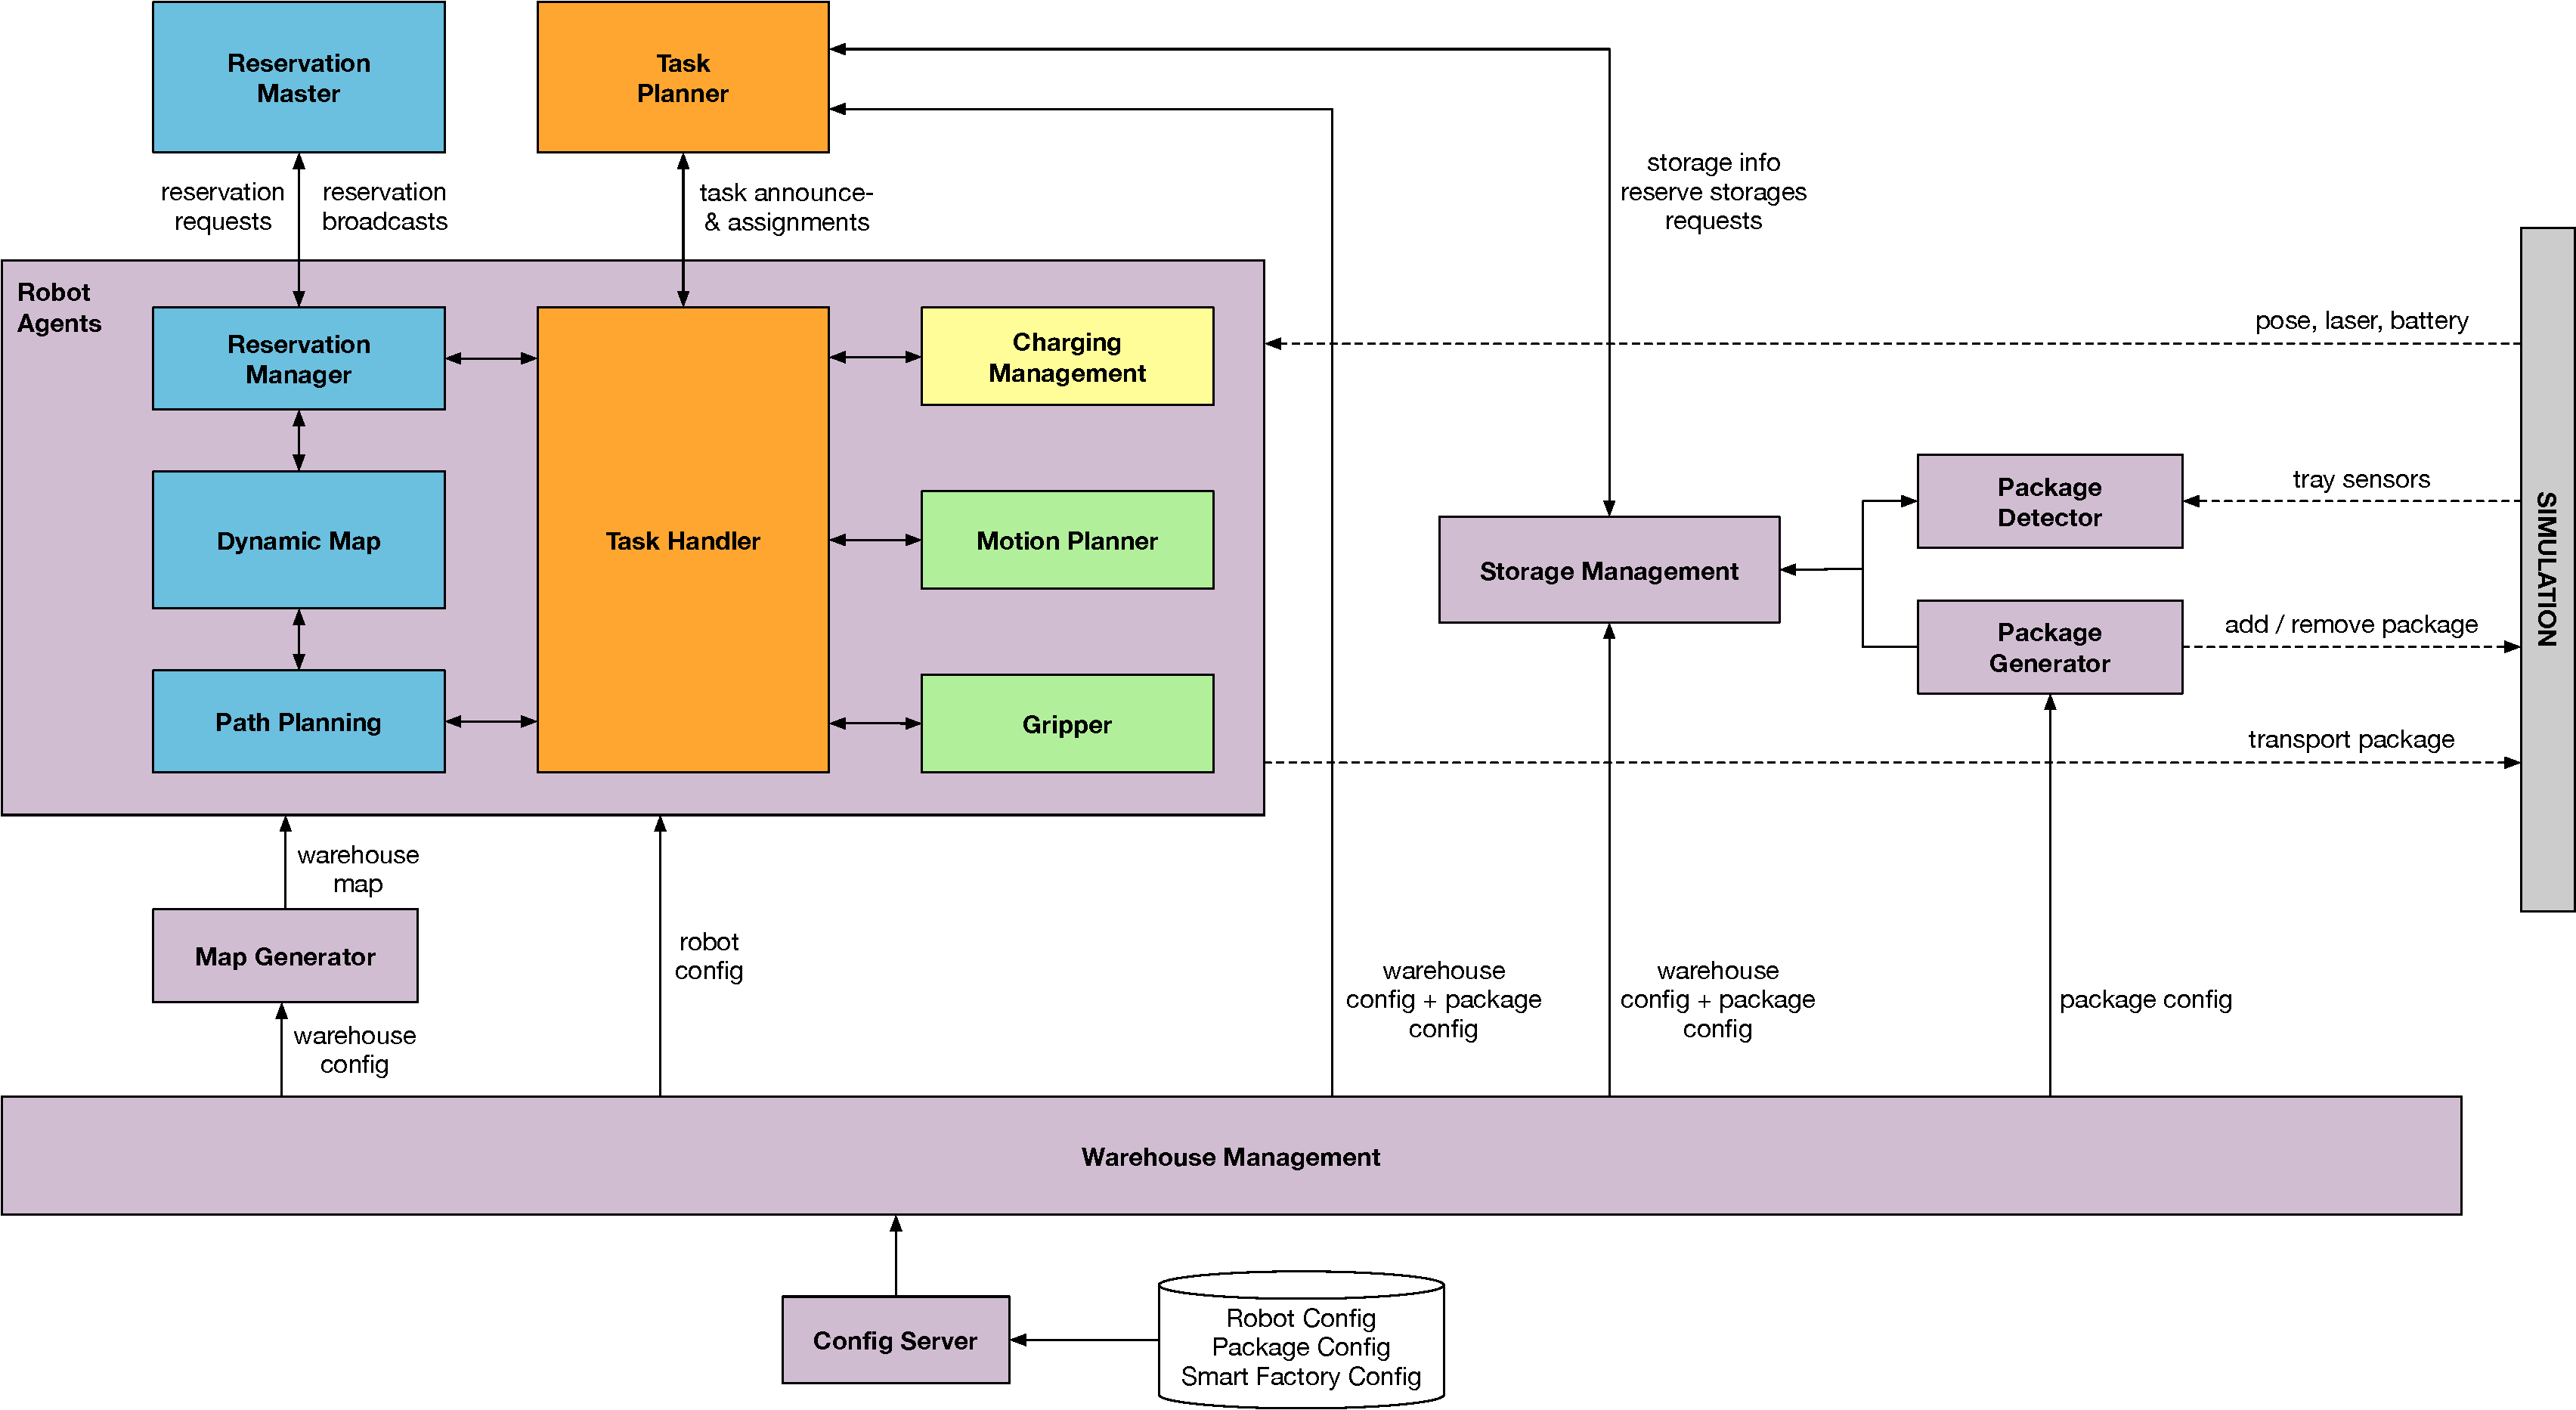
\includegraphics[width=0.45\textwidth]{resources/system_architecture}
	\caption{System Architecture}
	\label{fig:system_architecture}
\end{figure}

\subsection{Foundation}
\label{subsec:foundation}
This work builds on top of an existing warehouse simulation. The physical simulation is done in the Modular OpenRobots Simulation Engine \emph{MORSE}. An interface allows the communication with the Robot Operating System \emph{ROS} which runs all the system components.

The \emph{Warehouse Management} is the base of the system. It initializes most of the components (cf. config arrows in Figure \ref{fig:system_architecture}). It uses the \emph{Config Server} to read the robot, package and warehouse configurations and distributes them to the other nodes. Additionally, it collects robot status information and displays them in combination with the warehouse design in RViz.





\subsection{Task Planning}
\label{subsec:task_planning}
The task planning is done via a hybrid approach. This means that the task planning is done by two different types of components: a central \textit{Task Planner} and decentral \textit{Task Handler} in each of the robots.

The Task Planner is responsible for announcing new tasks to the robots, collecting their responses, picking the best suited robot and assigning tasks.

The Task Handler is responsible for computing the score of its robot for an announcement, answering to the Task Planner with that score and queuing of tasks assigned to its robot. The Task Handler is also responsible for keeping the robot charged.

There are two types of tasks: transportation tasks and charging tasks. Transportation tasks are announced and assigned by the Task Planner. In contrast charging tasks are not announced and instead assigned by the Task Handler of each robot without consulting the Task Planner.

When the Task Planner receives a request to assign a transportation task, it will announce the task to the robots and wait for them to answer.
The announcement includes all possible source and target trays for this task.
After receiving all answers or timing out, the Task Planner sorts the received answers by their score and assigns the task to the robot with the best score.

Each Task Handler receiving the task announcement computes the score for all possible source and target tray combinations and answers with the best score and the corresponding trays.

Since the score depends on the chosen source and target trays, the agent needs to estimate the following values: the duration to drive to the source tray $d_{source}$, the duration to drive to the target tray $d_{target}$ and the battery level after task completion $b$ in percent.

The overall duration $d$ is computed by:
$$d = d_{source} + d_{target} + d_{tasks}$$
where $d_{tasks}$ is the estimation of the time to finish all queued tasks.

As the estimated battery level itself would penalize the score linearly we instead use the factor $\alpha = f(b)$ computed by the Charging Management (cf. \compref{subsec:charging_management}).

The score $s$ for the chosen source and target tray can then be computed as:
$$ s = \frac{1}{\alpha} \cdot d$$
where $\alpha \in [0, 1]$.

A lower score therefore indicates a better combination of energy consumption and duration.


\subsection{Path Planning}
\label{subsec:path_planning}
Describing how the path planning works. At the end of the planning the paths need to be reserved, what's described in the coordination section.

\subsection{Coordination}
\label{subsec:coordination}
Describe how the coordination between the robots work. This chapter describes the ReserverationManager and the Arbiter (and explains why we use the Arbiter).

\subsection{Motion Planning}
\label{subsec:motion_planning}
The \emph{Motion Planner} is responsible for the linear and angular velocity of the robot. It utilizes a pid controller to calculate the angular velocity. There are cases where the pid controller doesn't provide an applicable solution. This includes sharp turns and turn arounds. For these cases the Motion Planner interrupts the pid controller and performs the rotation manually. The pid controller calculates the angular velocity based on the cross-track-error \emph{cte} with a sign to determine wether the robot is left or right off the track.

The linear velocity is calculated by subtracting an exponential translation of the cte from the maximum driving speed $v = v_{max} - min(\exp(cte^2-1), (v_{max}-v_{min}))$. It combines this with the value calculated from the distance to the target and uses the minimum of both. Finally the linear velocity is clamped between minimum and the maximum driving speed of the robot.

Whenever the robot reaches a waypoint of the path, the Motion Planner checks if the reservation for the next segment is active by comparing the departure time of the current waypoint with the real time. If the departure time is not passed yet, the robot waits at the waypoint.

For precise alignment and approach to the trays, the robot offers the functionality to precisely align towards a specified target and drive straight for a given distance.

\subsection{Charging Management}
\label{subsec:charging_management}
The \textit{Charging Management} is responsible for tracking the battery level, deciding when and where to charge, and computing the penalty factor for score calculation.

% charging behaviour -> when to go charging and when add charging tasks
When a robot is idle it still consumes energy. Therefore, it is possible for a robot to completely discharge while idling. 
To prevent this and always keep the charge at a reasonable level robots go charging when their charge is lower than a threshold.
The other case where robots should go charging is when the Task Handler receives a task announcement but can not find any combination of source and target tray with which the robot can finish the task with its remaining charge.
A robot always charges until its battery is fully charged.

% how to choose charging station
Ideally robots needing to charge should only drive short pathes to consume less charge. 
Therefore, the robots when needing to charge compute the nearest available charging station by checking if the space in front of the charging trays is reserved.
When a robot starts a charging task it computes the nearest charging station and reserves the path to it, with that it automatically reserves the charging station.

% how is penalty factor computed and why
The charging management is also responsible for computing the score factor which is dependent on the battery charge at the end of a task as mentioned in \compref{subsec:task_planning}.
We dont want the score influenced linearly by the charge for the complete charge interval. 
That is because for high charge levels we want the duration of the path being the deciding factor when comparing two possible solutions for a task.
Conversely when a robot will probably have low charge when ending the announced task we want robots with a longer paths but more charge left to be assigned the task.

We therefore created the following three-piece function $f(b) \in [0, 1]$, where $b$ is the battery level after task completion:
\[ 
f(b) = 
	\begin{cases}
		1.0,&\quad \text{if } b \geq u_t \\
		\frac{0.01 \cdot b^2 - (2 + 0.01 \cdot l_t) \cdot b - l_t}{100}, &\quad \text{if } u_t > b \geq l_t \\
		0.01 \cdot b, &\quad \text{otherwise} \\
	\end{cases}
\]
% describe upper and lower threshold
Where $u_t$ describes the charge at which the score should not yet be penalized and $l_t$ describes the charge under which the penalty is most severe.
In the system the values are set as $u_t = 50$ and $l_t = 35$.
% function is contiuous
This function has the benefit of being continuous and differentiable.


\subsection{Task Execution}
\label{subsec:task_execution}
% Describe how the Robot Agents operate (maybe call the section something like: Operation), how they work on the tasks, when they idle, ...
After we have discussed all the needed submodules we take a look at the execution of a task. Task execution is done by the \textit{Task Handler}.

It has access to the Path Planner, Reservation Manager, Motion Planner and Charging Management. In addition, it has a list, called queue, of tasks assigned by the Task Planner, as well as the task it is currently working on, called the current or active task.

The default state of the robot is idle. In this state it has neither an active task nor tasks waiting in its queue. If the robot has no active task or the active task is finished but one or more tasks are in the robots queue it will start the first task in the queue.

Depending on the type of the current task the execution consists of more or less steps. Important to note is that the robot only reserves paths that it is driving immediately after it receives the reservation and does not try to reserve paths further in the future. We decided on this behaviour because planning far into the future costs computation time and more importantly the environment is so uncertain that the probability that the plans have to be revised is high.

If the current task is a transportation task the Task Handler will go through the following steps:
\begin{enumerate}
	\item request from the Reservation Manager a reserved path from the current robot position to the tray where it is supposed to pick up the assigned package
	\item if it has received such a path hand it to the motion planner for driving
	\item when the robot arrives at the tray pick up the package
	\item when the package is loaded, request from the Reservation Manager a reserved path from the current position to the tray where it is supposed to drop the package off
	\item if it has received such a path hand it to the motion planner for driving
	\item when the robot arrives at the tray drop off the package
	\item when the the package is delivered, mark the task as finished
\end{enumerate}
For a charging task the execution procedure looks very similar:
\begin{enumerate}
	\item find the nearest free charging station
	\item request from the Reservation Manager a reserved path from the current robot position to the charging station
	\item if it has received such a path hand it to the motion planner for driving
	\item when the robot arrives at the charging station initiate the charging procedure
	\item when the battery is full, mark the task as finished
\end{enumerate}
% path replanning if necessary
While tasks are executed the Task Handler continuously checks if replanning is beneficial or necessary.

\subsection{Path Re-planning}
\label{subsec:path_replanning}
% replanning behavior -> when to replan and how does it work
The \textit{Path Replanning} is part of the Task Handler component.
Since all our reservations are based on estimations of the time a robot is in a specific area, it is possible that a robot is faster than anticipated. In this case another robot might be able to finish its current task earlier.
There are many situations where such an improvement is possible. 
because of time constraints we only consider the following situation for beneficial replanning:
When a robot leaves a tray earlier than estimated and planned for, another robot waiting to access that particular tray can access it earlier.

% describe behavior
When replanning for a task the Task Handler computes and reserves a new path through the Reservation Manager.
As long as the reservation is not yet granted it will continue with its current path.
When the new path is received the Task Handler hands it to the Motion Planner to drive and the replanning is complete.

% this behavior with one addition also allows us to recover from situations where a robot is to slow for its reservations and ends up outside of them
In the case of a robot being slower than planned for or more generally in the case of a robot not being in a reservation of its, replanning is not only beneficial but necessary.
The previously introduced behaviour with a simple addition can be used for this case as well. Instead of the robot continuing on its current path while the reservation is not yet granted, the robot places an emergency reservation on its current position and stops driving until it receives a new reserved path.

\subsection{Prototyping Environment}
\label{subsec:prototyping_environment}
Describe that we've used a prototyping environment to test all our path-planning and coordination algorithms in a simple and clean environment.

\section{Results}
\label{sec:results}
% Analysing the results is a very important validation for any project. But before that, one must define exact constraints for evaluation of these results. Also, the evaluations must be backed by scientific reasoning and empirical data. Therefore it is essential to first reason why particular parameters were chosen and how they are tested. Following sections explain the same.

\subsection{Evaluation Methodology}
\label{evaluation_methodology}
% mention evaluator as data collection unit, making easy evaluation of different configurations possible
% export as csv -> compare different configurations, compare basic parameters
% possible to simulate warehouse config to check for problems with tray placement etc.
The performance of our system was evaluated on two different maps (Table \ref{tab:maps}) of size 18x16 using different number of robots (1, 2, 4, 6, 8, 10 and 12) with the same characteristics. The simulation was repeated 3 times for each number of robots on each map. The simulation was finished when 40 transportation tasks were done. With the start of simulation the battery level of robots is randomized between 95 and 100.

For transportation tasks we sampled a) time stamps when a task is assigned, b) execution time of a task, c) time of driving to pick up, d) pick up time, e) time of driving to drop off, f) drop off time and g) battery level at the end of task. For charging tasks we sampled  a) time stamps when a task is assigned, b) execution time of a task, c) time of driving to charge, and d) charging time.

The performance of the system can be seen in following Figures. In Figure \ref{fig:delivery_time} we compare average package delivery time by number of robots for both maps. In Figure \ref{fig:trans_charg_idle} can be seen relative average time split of the states (transportation, charging and idle).

We tried to determinate the optimal amount of the robots for each map. Figure \ref{fig:time_to_finish_40_tasks} shows the average time to finish 40 tasks and figure \ref{fig:energy_consumption} presents energy consumption of the system for 40 tasks by number of the robots.

\subsection{Evaluation results and interpretation}

The graph \ref{No_of_robots_vs_average_time} shows average package delivery time increases with increase in number of robots.  Initially for one robots, a task can be executed as fast as possible, without any obstacles in between. As more robots participate in the simulation, robots need to avoid paths of other robots. This increases the coordination overhead which in turn leads into congestions. From robot 4 onwards, the package delivery time increases quite linearly as number of robots increase.

Similarly, in \ref{No_of_robots_vs_time_whiskers}, we can see that the variance between average delivery times is increased significantly. The reason for this can be again attributed to the coordination. Robots which reserve the direct path first will have the lowest travel time. On the contrary, robots reserving the path later will have to avoid pre reserved spots, thus taking a longer, non direct path. Compared to 15 \% varience in robot 1,  in robot 10, it almost becomes 25 \%.  

\begin{table}[h]
\caption{Maps Configuration}
\centering
\begin{tabular}{cccccc}
\hline
Map & Shape & \# Storage & \# Input             & \# Output & \# Charging \\ \hline
1   & 18x16 & 19         & 4                    & 5         & 8           \\
2   & 18x16 & 20         & 6                    & 8         & 8           \\ \hline
    &       &            & \multicolumn{1}{l}{} &           &            
\end{tabular}
\label{tab:maps}
\end{table}


\begin{figure}[h]
	\centering
	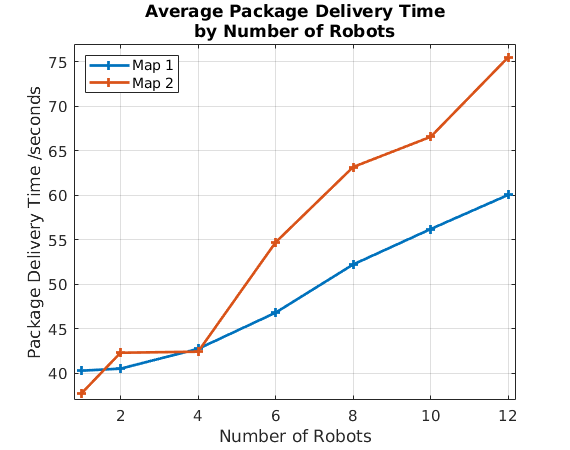
\includegraphics[width=0.45\textwidth]{resources/Graphs-paper/graph2.png}
	\caption{Average Package Delivery Time by Number of Robots}
	\label{fig:delivery_time}
\end{figure}

\begin{figure}[h]
	\centering
	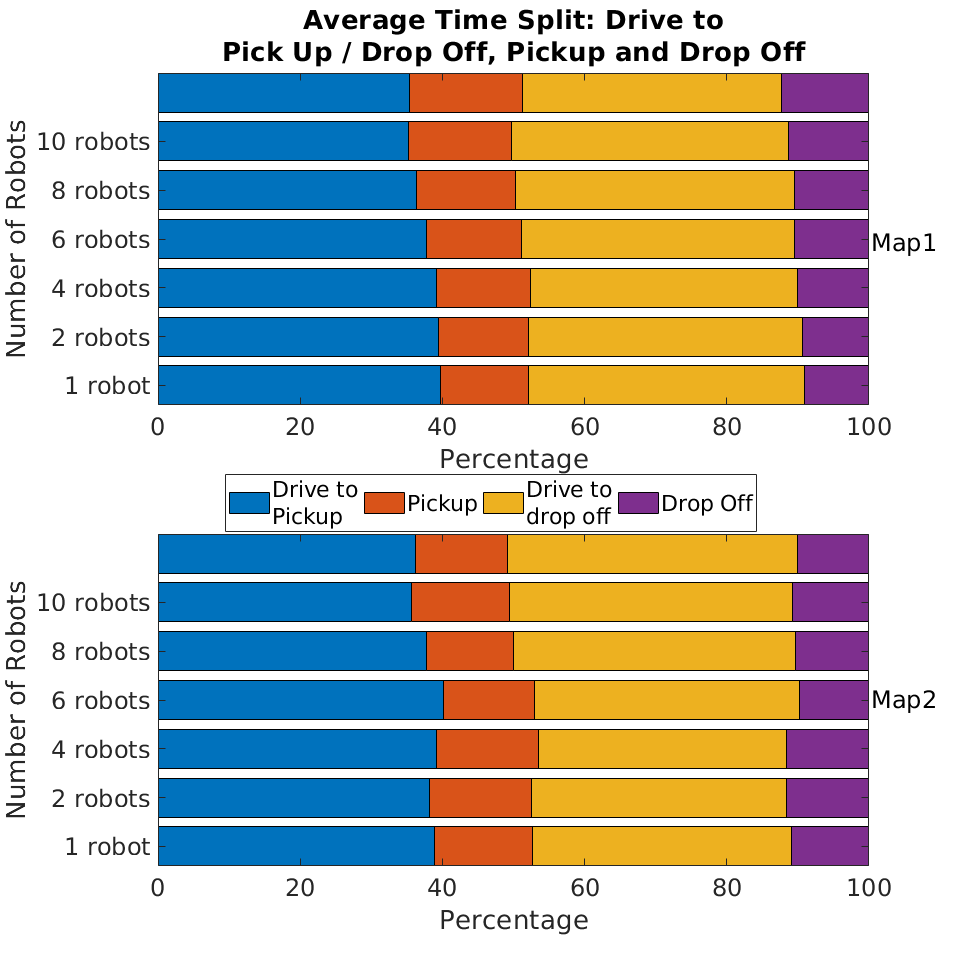
\includegraphics[width=0.45\textwidth]{resources/Graphs-paper/graph3_2.png}
	\caption{Average time split: drive to pick up / dropp off, pick up and drop off}
	\label{fig:drive_pickup_dropoff}
\end{figure}

\begin{figure}[h]
	\centering
	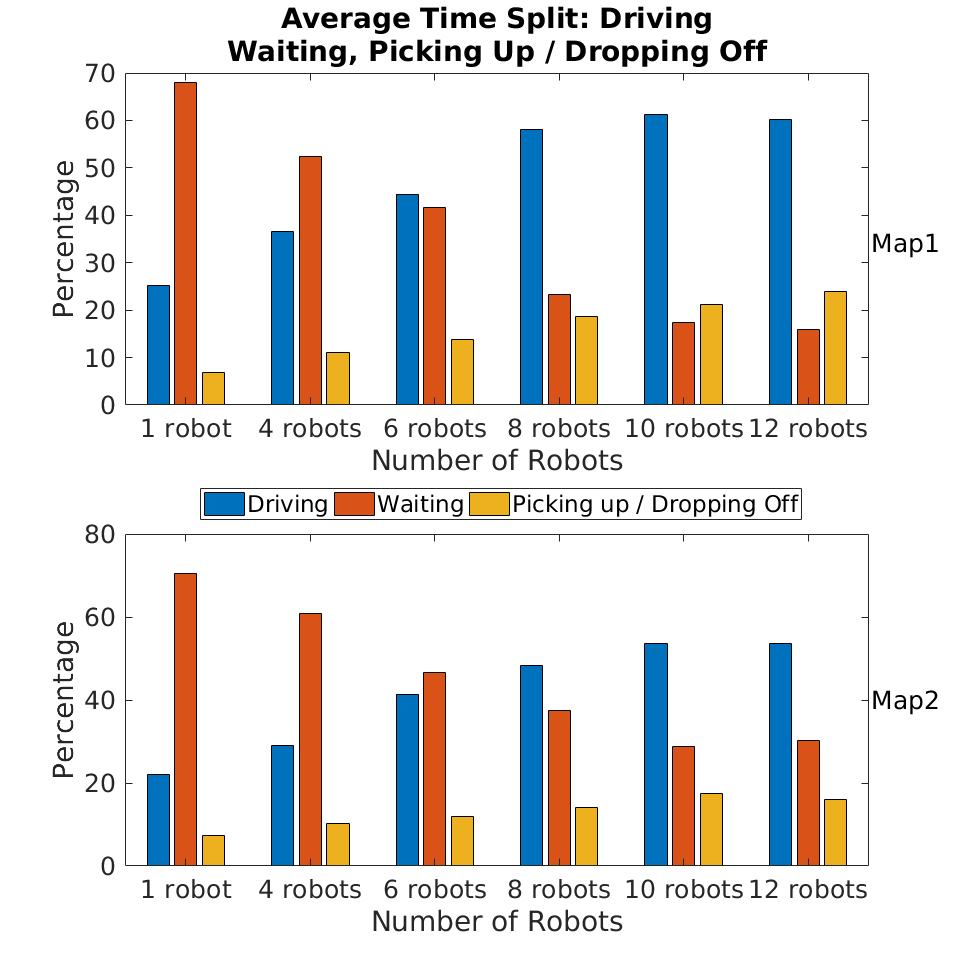
\includegraphics[width=0.45\textwidth]{resources/Graphs-paper/graph4.png}
	\caption{Average Package Delivery Time by Number of Robots}
	\label{fig:delivery_time}
\end{figure}

\begin{figure}[h]
	\centering
	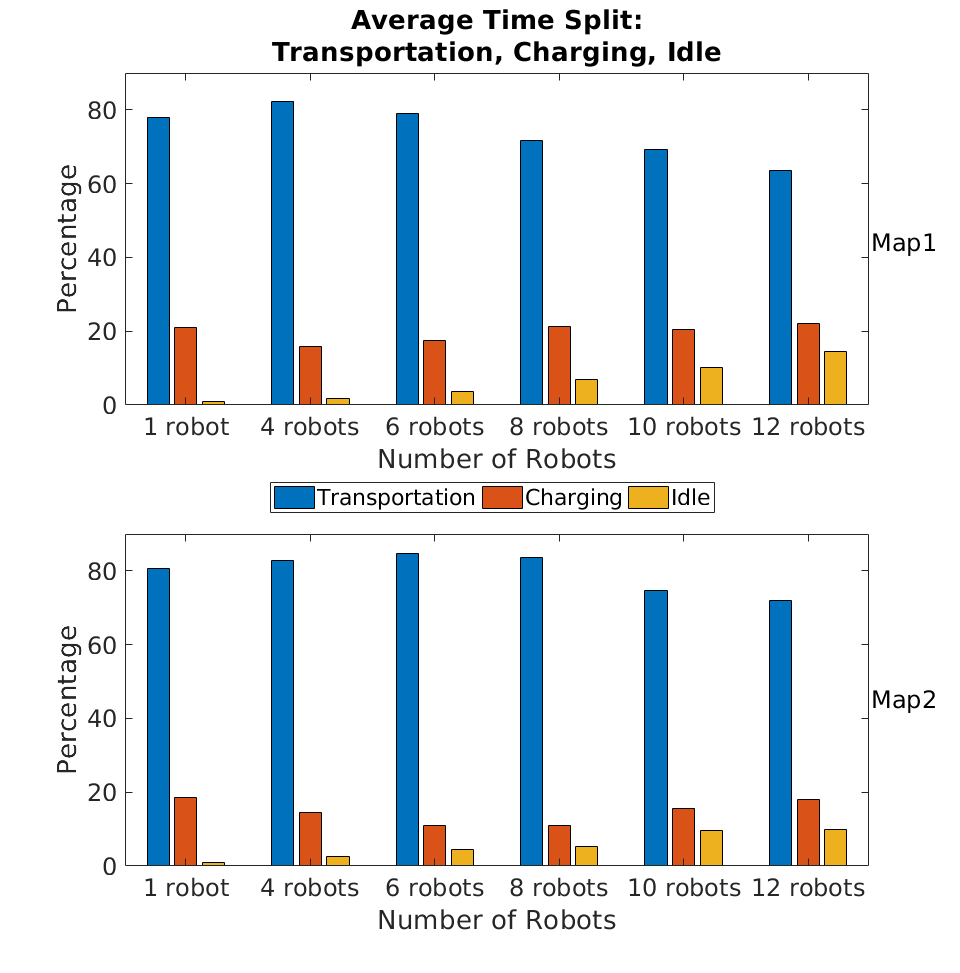
\includegraphics[width=0.45\textwidth]{resources/Graphs-paper/graph7.png}
	\caption{Average time split: transportation, charging, idle}
	\label{fig:trans_charg_idle}
\end{figure}

\begin{figure}[h]
	\centering
	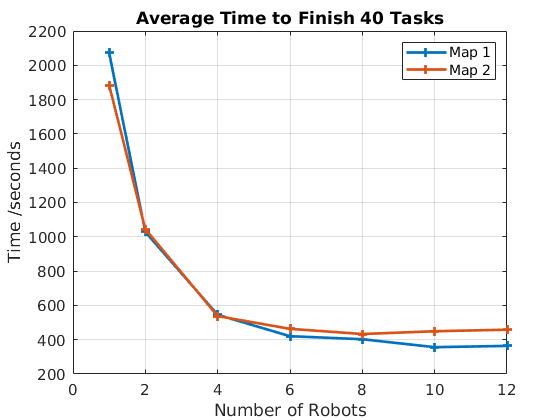
\includegraphics[width=0.45\textwidth]{resources/Graphs-paper/graph6.png}
	\caption{Average time to finish 40 tasks}
	\label{fig:time_to_finish_40_tasks}
\end{figure}

\begin{figure}[h]
	\centering
	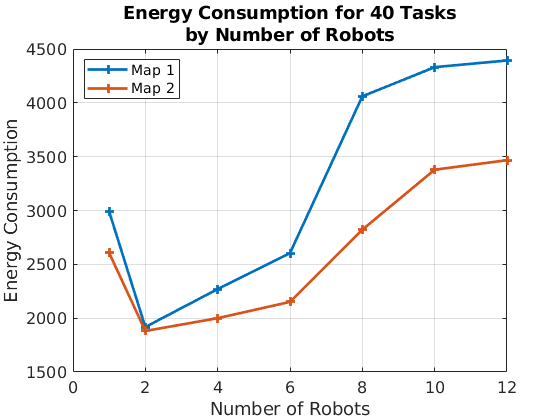
\includegraphics[width=0.45\textwidth]{resources/Graphs-paper/graph8.png}
	\caption{Energy consumption for 40 tasks by number of robots}
	\label{fig:energy_consumption}
\end{figure}


In graph \ref{No_of_robots_vs_average_time_all_taks}, we can however see the positive effect of adding number of robots. The total time to finish 40 tasks drops by more than 60 \% when we use 4 robots instead of 1. This certifies the goal of the system, that the multi robot collaboration significantly improves the performance of the system. Furthermore, we can see the performance improvement is incremental from 4 robots onwards. As number of robots is more, and available space remains the same, robots cancel the positive effect of collaboration with negative effect of congestion. At 10 robots, we can see increase in time.

In graph \ref{fig:drive_pickup_dropoff} we can see what percent of time the robot has spent in various activities. As expected, the robot spends most of it's time in driving, either to pickup or dropoff. However, if we consider results of Map 1 in \ref{fig:delivery_time}, the combined percent time taken for pickup and dropoff is increased from 9 \% for 1 robot to around 22 \% for 12 robots.  As the trays available for pickup and dropoff are limited (4 and 5 respectively), robots have to coordinate among themselves to get a space in front of the trays. This creates a bottleneck for robots and often results in congestions. 


To find an even split between the times, the aforementioned parameters were  tweaked for optimum values which we can see in map2 \ref{fig:drive_pickup_dropoff}. Here, the distribution of time split almost similar even if number of robot agents was increased.  

%therefore at one point the time increases
%to add after new graphs









% needed in second column of first page if using \IEEEpubid
%\IEEEpubidadjcol

% An example of a floating figure using the graphicx package.
% Note that \label must occur AFTER (or within) \caption.
% For figures, \caption should occur after the \includegraphics.
% Note that IEEEtran v1.7 and later has special internal code that
% is designed to preserve the operation of \label within \caption
% even when the captionsoff option is in effect. However, because
% of issues like this, it may be the safest practice to put all your
% \label just after \caption rather than within \caption{}.
%
% Reminder: the "draftcls" or "draftclsnofoot", not "draft", class
% option should be used if it is desired that the figures are to be
% displayed while in draft mode.
%
%\begin{figure}[!t]
%\centering
%\includegraphics[width=2.5in]{myfigure}
% where an .eps filename suffix will be assumed under latex, 
% and a .pdf suffix will be assumed for pdflatex; or what has been declared
% via \DeclareGraphicsExtensions.
%\caption{Simulation Results}
%\label{fig_sim}
%\end{figure}

% Note that IEEE typically puts floats only at the top, even when this
% results in a large percentage of a column being occupied by floats.


% An example of a double column floating figure using two subfigures.
% (The subfig.sty package must be loaded for this to work.)
% The subfigure \label commands are set within each subfloat command, the
% \label for the overall figure must come after \caption.
% \hfil must be used as a separator to get equal spacing.
% The subfigure.sty package works much the same way, except \subfigure is
% used instead of \subfloat.
%
%\begin{figure*}[!t]
%\centerline{\subfloat[Case I]\includegraphics[width=2.5in]{subfigcase1}%
%\label{fig_first_case}}
%\hfil
%\subfloat[Case II]{\includegraphics[width=2.5in]{subfigcase2}%
%\label{fig_second_case}}}
%\caption{Simulation results}
%\label{fig_sim}
%\end{figure*}
%
% Note that often IEEE papers with subfigures do not employ subfigure
% captions (using the optional argument to \subfloat), but instead will
% reference/describe all of them (a), (b), etc., within the main caption.


% An example of a floating table. Note that, for IEEE style tables, the 
% \caption command should come BEFORE the table. Table text will default to
% \footnotesize as IEEE normally uses this smaller font for tables.
% The \label must come after \caption as always.
%
%\begin{table}[!t]
%% increase table row spacing, adjust to taste
%\renewcommand{\arraystretch}{1.3}
% if using array.sty, it might be a good idea to tweak the value of
% \extrarowheight as needed to properly center the text within the cells
%\caption{An Example of a Table}
%\label{table_example}
%\centering
%% Some packages, such as MDW tools, offer better commands for making tables
%% than the plain LaTeX2e tabular which is used here.
%\begin{tabular}{|c||c|}
%\hline
%One & Two\\
%\hline
%Three & Four\\
%\hline
%\end{tabular}
%\end{table}


% Note that IEEE does not put floats in the very first column - or typically
% anywhere on the first page for that matter. Also, in-text middle ("here")
% positioning is not used. Most IEEE journals use top floats exclusively.
% Note that, LaTeX2e, unlike IEEE journals, places footnotes above bottom
% floats. This can be corrected via the \fnbelowfloat command of the
% stfloats package.



\section{Conclusion}
FROM CAN:
\\
A brief summary of your system, what was the problem, how you achieved, your objectives, and your methodologies you used very very briefly. Then again very briefly share your finding (the discussion you made). Finally, you will conclude with the possible extensions / changes to improve the performance, basically the future works. You can find more about the templates of IEEE on the internet.




% if have a single appendix:
\appendix[Class Diagram]

Here I would like to see your final class diagram. It doesn’t require any description (unless it is complicated). It will be sufficient and necessary to mention at least once inside the methodology part that your class diagram is attached as an appendix. Also give figure caption to it.


% or
%\appendix  % for no appendix heading
% do not use \section anymore after \appendix, only \section*
% is possibly needed

% use appendices with more than one appendix
% then use \section to start each appendix
% you must declare a \section before using any
% \subsection or using \label (\appendices by itself
% starts a section numbered zero.)


% Can use something like this to put references on a page
% by themselves when using endfloat and the captionsoff option.
\ifCLASSOPTIONcaptionsoff
  \newpage
\fi



% trigger a \newpage just before the given reference
% number - used to balance the columns on the last page
% adjust value as needed - may need to be readjusted if
% the document is modified later
%\IEEEtriggeratref{8}
% The "triggered" command can be changed if desired:
%\IEEEtriggercmd{\enlargethispage{-5in}}

% references section

% can use a bibliography generated by BibTeX as a .bbl file
% BibTeX documentation can be easily obtained at:
% http://www.ctan.org/tex-archive/biblio/bibtex/contrib/doc/
% The IEEEtran BibTeX style support page is at:
% http://www.michaelshell.org/tex/ieeetran/bibtex/
%\bibliographystyle{IEEEtran}
% argument is your BibTeX string definitions and bibliography database(s)
%\bibliography{IEEEabrv,../bib/paper}
%
% <OR> manually copy in the resultant .bbl file
% set second argument of \begin to the number of references
% (used to reserve space for the reference number labels box)
\begin{thebibliography}{1}
\bibitem{IEEEhowto:kopka}
H.~Kopka and P.~W. Daly, \emph{A Guide to \LaTeX}, 3rd~ed.\hskip 1em plus
  0.5em minus 0.4em\relax Harlow, England: Addison-Wesley, 1999.
\bibitem{AStar}
Hart, Peter E., Nils J. Nilsson, and Bertram Raphael. "A formal basis for the heuristic determination of minimum cost paths." IEEE transactions on Systems Science and Cybernetics 4.2 (1968): 100-107.
\bibitem{ThetaStar}
Nash, Alex, et al. "Theta*: Any-angle path planning on grids." AAAI. Vol. 7. 2007.
\bibitem{Roadmaps}
Kavraki, Lydia, Petr Svestka, and Mark H. Overmars. Probabilistic roadmaps for path planning in high-dimensional configuration spaces. Vol. 1994. Unknown Publisher, 1994.
\bibitem{RRT}
LaValle, Steven M. "Rapidly-exploring random trees: A new tool for path planning." (1998).
\bibitem{RRTStar}
Karaman, Sertac, and Emilio Frazzoli. "Incremental sampling-based algorithms for optimal motion planning." Robotics Science and Systems VI 104.2 (2010).
\bibitem{ThetaStarRRTStar}
Palmieri, Luigi, Sven Koenig, and Kai O. Arras. "Rrt-based nonholonomic motion planning using any-angle path biasing." 2016 IEEE International Conference on Robotics and Automation (ICRA). IEEE, 2016.
\bibitem{DMA}
Desaraju, Vishnu R., and Jonathan P. How. "Decentralized path planning for multi-agent teams in complex environments using rapidly-exploring random trees." 2011 IEEE International Conference on Robotics and Automation. IEEE, 2011.
\end{thebibliography}

%\vfill

% Can be used to pull up biographies so that the bottom of the last one
% is flush with the other column.
%\enlargethispage{-5in}



% that's all folks
\end{document}


\grid
